\section*{Kursbeschreibung}
\sectionauthor{Philipp Arras, Gordian Edenhofer}
Information ist ein allgegenwärtiger Begriff. Jede*r hat ein Gefühl dafür, was es heißt Informationen zu bekommen, mehr Informationen zu haben als jemand anderes und aus Informationen zu lernen.
Informationstheorie definiert Information auf eine scharfe mathematische Art und Weise, kann alle wesentlichen Aspekte des Sprachgebrauchs abbilden und ermöglicht es darüber hinaus, Informationen in Bits zu messen.

Der Kurs führt zunächst in die Informationstheorie und die bayessche Wahrscheinlichkeitsrechnung ein.
Mithilfe dieser Sichtweise erklärt der Kurs, was es heißt durch Informationen zu lernen und was es in diesen Kontext bedeutet \enquote{optimal} zu lernen.
Als Anwendung dieser Theorie beschäftigt sich der Kurs mit bildgebenden Verfahren von wissenschaftlichen Messgeräten, wie etwa Computertomographen (CT) oder Radioteleskopen.
Anders als herkömmliche Kameras, vermessen diese Instrumente das aufzunehmende Objekt nur indirekt.

Für die meisten dieser Anwendungen ist es nicht möglich \enquote{perfekt} aus den Messdaten zu Lernen, weshalb Näherungslösungen benutzt werden müssen.
Hierfür vermittelt der Kurs Grundlagen in Linearer Algebra und Analysis.
Im Kurs erarbeiten sich die Teilnehmenden in Gruppenarbeit am Computer, solche Näherungslösungen zu berechnen.

Das Kursziel ist es, dass die Teilnehmenden selbständig ein bildgebendes Verfahren für ein Messinstrument in Python schreiben, um damit ein aus den Rohdaten eines CT-Scans oder den Radioteleskopdaten vom Schwarzen Loch M87* ein Bild zu rekonstruieren.
Im Vorfeld der Akademie soll ein Vortrag vorbereitet werden mit hierzu bereitgestellter passender Literatur.
Zusätzlich wird vorab Material zur Verfügung gestellt anhand dessen sich Teilnehmende mit der Programmiersprache Python vertraut machen sollen.

\section{Einleitung}
\sectionauthor{Natalie Teplitska, Leo Bergmann}

Unser Kurs beschäftigte sich mit der computergestützten Gewinnung von Bildern aus Rohdaten.
Bei vielen Untersuchungsobjekten in der Physik und Medizin benötigt man bildgebende Verfahren, weil Messungen nur indirekt möglich sind.
Daher erarbeiteten wir uns notwendige mathematische Konzepte der Informationstheorie (IT) und wandten diese auf ein Beispiel aus der Radioastronomie und auf Computertomografie an.

Da wir Theorien aus diversen Anwendungsbereichen benötigten, haben wir uns diese bereits vor der Akademie im mithilfe vom Postern angeeignet und innerhalb der ersten Tage den anderen vorgestellt.
Dazu hielt jede:r einen 20-minütigen Vortrag auf Grundlage des Posters innerhalb eines durchdachten Rotationssystems.
Die Poster wurden am ersten Tag aufgehängt und weckten somit das Interesse der anderen Kurse und personalisierten den Standort.

Diese Fülle an Informationen vervollständigten Gordian und Philipp mit ihrem Wissen und ihrer Erfahrung in mehreren Input-Sessions, welche vornehmlich die erste Woche in Anspruch nahmen
Wir erhielten, alternierend von Gordian und Philipp eine Einführung in die IT, Radioastronomie, Staubtomografie und ganz viel Mathematik.

\begin{figure}
    \centering
    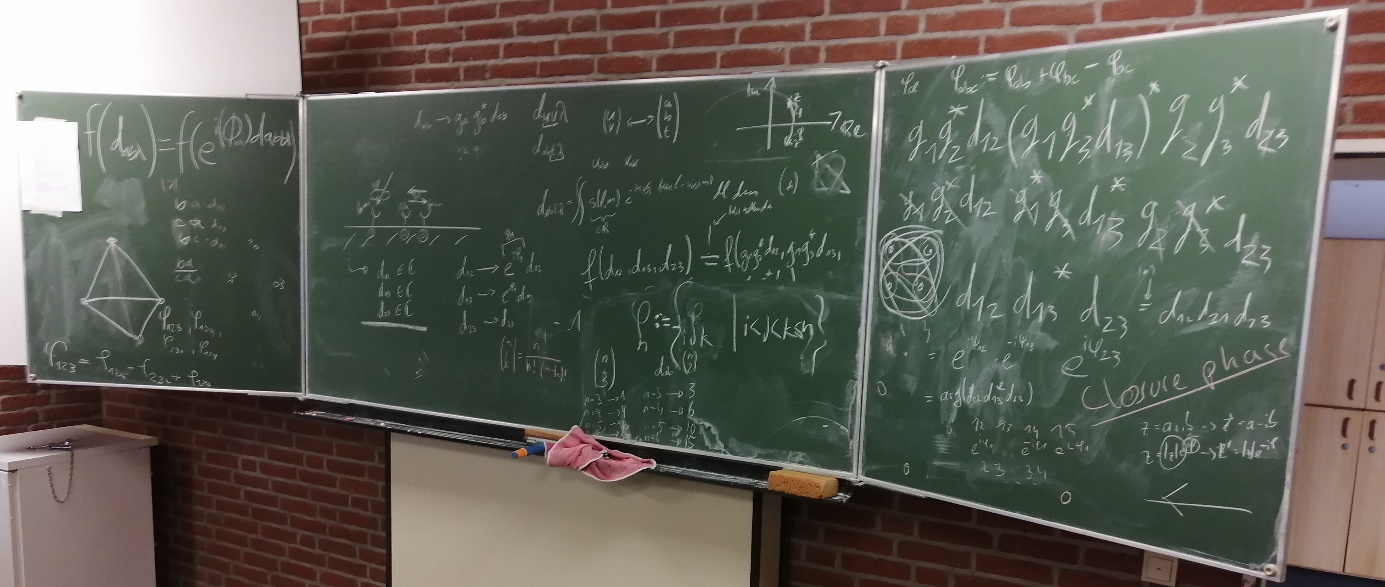
\includegraphics[width=0.8\textwidth]{k4.2/tafelbild.png}
    \caption{Tafel-Chaos}
\end{figure}

\begin{figure}
    \centering
	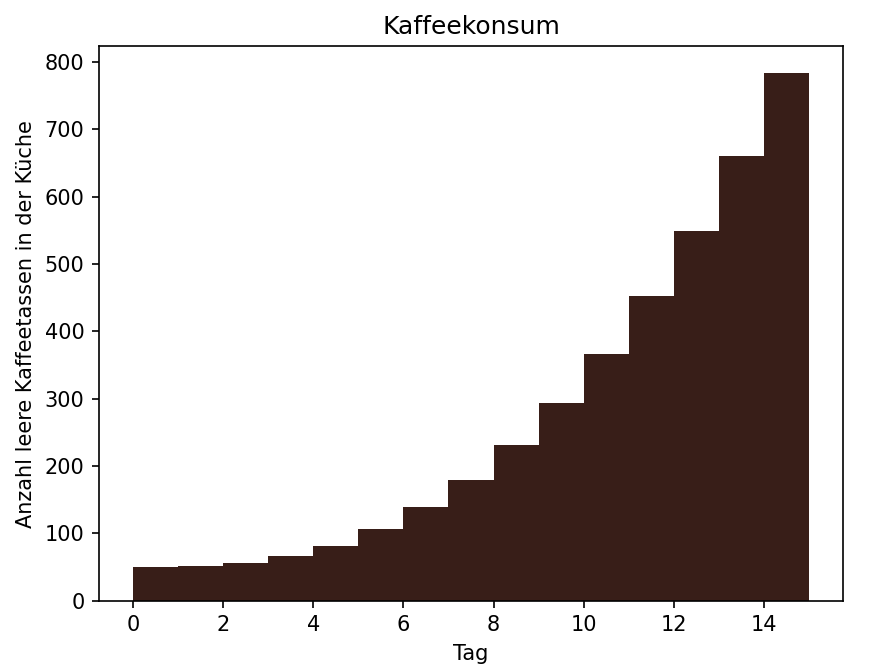
\includegraphics[width=0.5\textwidth]{k4.2/kaffee.png}
	\caption{Kaffeekonsum}
    \label{k4.2.fig.kaffee}
\end{figure}

In der zweiten Woche arbeiteten wir an eigenen Projekten.
Je zwei Projektteams beschäftigen sich mit Datenverarbeitung aus der Radioastronomie und der Computer-Tomographie.
Das fünfte Projektteam erarbeitete weitere mathematische Konzepte, welche für beide Projekte essenziell waren.
Die Projektarbeit gab uns die Möglichkeit, unser Wissen eigenständig anzuwenden.
Allerdings mussten besonders gegen Ende der Akademie Teile der Projektarbeit außerhalb der Kurse erledigt werden, was sich im allgemeinen Kaffeekonsum der Akademie niederschlug (siehe \cref{k4.2.fig.kaffee}).
Es war ein hartes Stück Arbeit, welches wir mit Python und viel Kaffee jedoch schlussendlich in den Griff bekamen.
Und das Ergebnis kann sich in jedem Fall sehen lassen.
